% !TeX spellcheck = en_US
%===================================== CHAP 3 =================================

\chapter{Basic Theory}

Common to all the attack vectors described in the previous chapter is that the attacker rely on background knowledge, often also called auxiliary information, to perform their linkage attacks. Protecting a database against this threat has long been a major challenge in database design. Already back in 1977 Tore Dalenius \cite{dalenius1977towards} defined a desideratum for data privacy which says that: \begin{quote}
	Access to the published data should not enable the adversary to learn anything extra about target victim compared to no access to the database, even with the presence of any adversary’s background knowledge obtained from other sources.
\end{quote} 

This privacy goal was rejected by Cynthia Dwork, who showed the general impossibility of Dalenius' goal due to the existence of auxiliary information. Instead she chose to formulate a probabilistic privacy goal, which places an upper bound on how much the risk of privacy breach can increase by participating in a database.

%In a world where massive amounts of sensitive personal data are being collected, attacks on the individual's privacy are becoming more and more of a threat. One type of attack is the identification of an individual's personal information from massive data sets, such as people's movie ratings from the Netflix data set\cite{narayanan2008robust}, and the medical records of a former governor of Massachusetts\cite{barth2012re}. These types of privacy breaches may lead to the unwanted discovery of a person's embarrassing information, and could also lead to the theft of an individual's private data or identity.  
%
%Many different approaches have been tried by data custodians to privatize the data they hold, such as removing any columns containing Personally Identifiable Information (PII), anonymizing the data by providing k-anonymity protection\cite{sweeney2002k}, or perform group based anonymization through l-diversity\cite{machanavajjhala2007diversity}. All of these methods mentioned have been proved to be susceptible in some way or form to attacks \cite{ganta2008composition}. Motivated by these shortcomings, a researcher at Microsoft came up with a data theoretical framework called differential privacy, which operates off a solid mathematical foundation and have strong theoretical guarantees on the privacy and utility of the released data.

\section{Differential Privacy}
\label{section:differential_privacy}
The term "differential privacy" was defined by Dwork as a description of a promise, made by a data holder to a data subject: "You will not be affected, adversely or otherwise, by allowing your data to be used in any study or analysis, no matter what other studies, data sets, or information sources, are available." \cite{dwork2013algorithmic}
In an ideal situation, databases which implement differential privacy mechanisms can make confidential data widely available for accurate data analysis, without resorting to data usage agreements, data protection plans, or restricted views. Nevertheless, the Fundamental Law of Information Recovery states that overly accurate answers to too many questions will destroy privacy in a spectacular way \cite{dwork2013algorithmic}, meaning that data utility will eventually be consumed.

\subsection{Definition of Differential Privacy}
The classic example for explaining a security breach is the case of Mr White: Suppose you have access to a database that allows you to compute the income of all residents in a specified area. If you knew that Mr White was going to move, simply querying the database before and after his relocation would allow you to deduce his income. 

\begin{definition} The distance of two datasets, $d(D_1, D_2)$, denotes the minimum number of sample changes that are required to change $D_1$ into $D_2$.
\end{definition}

Formally, differential privacy is defined as follows:
A randomized function $M$ gives $\epsilon$-differential privacy if for all data sets $D_1$ and $D_2$ where $d(D_1, D_2)=1$, and all $S\subseteq Range(M)$,
\begin{eqnarray} \label{DiffPrivDef}
 Pr[M(D_1)\in S]\leq \mathrm{e}^{(\epsilon)}\times Pr[M(D_2)\in S]
 \end{eqnarray}

That is, the presence or absence of a particular record should not affect the probability of any given output of $M(D)$ by more than some multiplicative factor. 

Informally, the presence or absence of a single record in a database should not have a noticeable impact on the output of any queries sent to it. Though the existence of the database itself might allow attackers to learn information about a person, opting out of the database will not significantly help reduce the risk of information disclosure. Conversely, participating in the database does not significantly increase the risk of disclosure either, thus fulfilling Dworks promise quoted in the beginning of Section \ref{section:differential_privacy}.

Privacy preserving data analysis platforms such as PINQ\cite{mcsherry2009PINQ}, Airavat\cite{roy2010airavat} and Fuzz\cite{Haeberlen2011fuzz} have all implemented features such as privacy budgeting and noise mechanisms to compute useful queries while fulfilling Equation \ref{DiffPrivDef}.

\subsection{Privacy Budget}
The quotient $\frac{Pr[M(D_1)\in S]}{Pr[M(D_2)\in S]}$ measures the extent to which an attacker can ascertain the difference between the two datasets\cite{abowd2008protective}. Sarathy and Muralidhar\cite{Sarathy2011evaluating} calls this ratio the ''knowledge gain ratio''. Differential privacy requires that this ratio is limited to $e^\epsilon$. This is because as the ratio grows larger, an attacker can determine with greater probability that the query result was obtained from one dataset over the other.

Privacy budgeting was introduced to limit the amount of information a data analyst can obtain about any individual with data records in the dataset. The data analysis platform will track every query to ensure that both individual queries and aggregation queries do not exceed the given budget. This privacy standard forbids further queries to the database once the budget has been consumed. 

\todo{Formalize why additive privacy budget works.}

When making a practical implementation, the $\epsilon$ value represents the privacy budget of the dataset. The budget value is set by the data analyst, but as it was shown in \cite{Sarathy2011evaluating} that the attacker's knowledge gain rises exponentially with the rising number of queries. Setting a high value for $\epsilon$ will have a measurable impact on data privacy. 


\subsection{Noise Mechanisms}
Given a target function $f$ to compute on a database $D$, it is necessary to design a randomized function $M$ which fulfills Equation \ref{DiffPrivDef} while yielding a useful approximation to the true $f$. This randomized function $M$ can be created by adding noise to the computation of $f$. There are many different mechanisms for applying this noise, but the two most common are the Laplace mechanism and the Exponential mechanism. 

\subsubsection{Laplace Mechanism}
The Laplace mechanism involves adding random noise which follows the Laplace statistical distribution. The Laplace distribution centered around zero has only one parameter, its scale $b$, and this is proportional to its standard deviation. 
\begin{eqnarray} \label{LaplaceDisDef}
Lap(x|b) = \frac{1}{2b} exp (-\frac{|x|}{b})
\end{eqnarray}
When using the Laplace mechanism it is necessary to choose a suitable value for the parameter $b$. Increasing values of $b$ results in increased noise variance. The scale of $b$ is naturally dependent on the privacy parameter $\epsilon$, and also on the effect the presence or absence of a single record can have on the output of function $f$. This risk is called the sensitivity of the function, and is defined mathematically as:
\begin{eqnarray} \label{LaplaceMecDef}
\Delta f=\underset{D_1,D_2}{max}||\mathit{f(D_1)}-\mathit{f(D_2)}||_{1}
 \end{eqnarray}
 \missingfigure[figwidth=6cm]{Picture showing the laplacian distribution} \unsure{Not sure if we need the pic. Alex: I think we do.}]

This equation states that the sensitivity $\Delta f$ is the maximum difference in the values that the function $f$ may take on any pair of databases that differ on only one row. Dwork proved that adding a noise drawn from $Lap(\Delta f/\epsilon)$ to a query, $\epsilon$-differential privacy\cite{dwork2013algorithmic} is guaranteed. 

\todo{add a section explaining that while it would seem that sensitivity is would often be high, some functions like count are naturally low sensitivity, and that steps such as clamping can be taken to reduce sensitivity}

\subsubsection{Exponential Mechanism}
The exponential mechanism proposed by McSherry and Talwar \cite{mcsherry2007} is a method for selecting one element from a set, and is commonly used if a non-numeric value query is used. An example would be: "What is the most common eye color in this room?". Here it would not make sense to perturb the answer by adding noise drawn from the Laplace distribution. The idea of the exponential mechanism is to select the output from all the possible answers at random, with the probability of selecting a particular output being higher for those outputs that are "closer" to the true output. 

More formally, let A be the range of of possible outputs for the query function $f$. Also, let $u_f(D,a)$ be a utility function that measures how good an output $a\in A$ is as an answer to the query function $f$ given that the input dataset is $D$ (Note that higher values of $u_f$ represents better outputs). The sensitivity function will then be defined as the maximum possible change in the utility function's value $u_f$ due to the addition or removal of one person's data from the input, i.e: \newline
\textbf{Definition 4}: the sensitivity of score function $u_f$ is defined as
\begin{eqnarray} \label{ExpoMecDef}
S(u_f) = \underset{d(D_1,D_2)=1,a\in A}{max}||u_f(D_1, a)-u_f(D_2,a)||
 \end{eqnarray}
 
 `
 \section{Logistic Regression}
 
 Logistic regression is a popular probability model developed by D.R Cox in 1958. The most basic form is used to predict a binary response based on a set of features.
 
 \begin{eqnarray} 
 h_{\theta}(x) = \theta^Tx = \sum_{i=0}^n \theta_i x_i, \nonumber
 \end{eqnarray}
 
 The logistic regression model is
  \begin{eqnarray} 
 p(y = ±1|\textbf{x, w}) = \sigma(y \textbf{w}^T \textbf{x}) = \frac{1}{1 + exp(−y \textbf{w}^T \textbf{x})}
  \end{eqnarray}
 (1)
 It can be used for binary classification or for predicting the certainty of a binary outcome. See Cox  and Snell (1970) for the use of this model in statistics. This note focuses only on computational issues related
 to maximum-likelihood or more generally maximum a-posteriori (MAP) estimation. A common
 prior to use with MAP is:
 p(w) ∼ N (0, λ−1  I) (2)
 Using λ > 0 gives a “regularized” estimate of w which often has superior generalization performance,
 especially when the dimensionality is high (Nigam et al., 1999).
 Given a data set (X, y) = [(x1, y1), ...,(xN , yN )], we want to find the parameter vector w which
 maximizes:
 \begin{eqnarray} 
 log(1 + exp(−y_i \textbf{w}^T \textbf{x}_i)) - \frac{\lambda}{2} \textbf{w}^T \textbf{w}
\end{eqnarray}
 The gradient of this objective is
 \begin{eqnarray} 
 g = \Delta_w l (\textbf{w}) = \sum_{i}^{} (1 - \sigma(y_i \textbf{w}^T	\textbf{x}_i)) y_i \textbf{x}_i - \lambda \textbf{w}
\end{eqnarray} 

When m, the number of observations or training examples, is not large enough compared to n, the
number of feature variables, simple logistic regression leads to over-fit. A standard technique to prevent over-fitting is regularization, in which an extra term that penalizes large weights is added to the average logistic loss function. The $l_2$-regularized logistic regression problem is
\begin{eqnarray}
minimize:	  l_{avg}(v,w)+ \lambda||w||^2_2 = (1/m) \sum_{i=1}^{m} f(w^T a_i +vb_i) + \lambda \sum_{i=1}^{n} w_i^2
\end{eqnarray}
Here $\lambda > 0$ is the regularization parameter, used to control the trade-off between the average logistic loss and the size of the weight vector, as measured by the $l_2$-norm. The objective function in this logistic regression problem is smooth and convex, and can be minimized by standard gradient descent.


\subsection{Sensitivity of Logistic Regression}

\todo{reference kamalikas paper for logres senstivity}

\todo{reference pathaks paper for sensitivity of aggregation process}

 \section{Programming Frameworks Used [Rename]}

 \subsection{JADE}
 The Java Agent framework for Distance learning Environments(JADE) is a middleware which facilitates the development of multi-agent systems. An application based on JADE is made of a set of components called agents, where each one has an unique name. Agents execute tasks and interact by exchanging messages between each other. Agents execute on top of a platform that provides them with basic services such as message delivery. A platform is composed of one or more containers, where the containers can be executed on different hosts thus achieving a distributed platform. The Main container is a special container which exists in the platform, as it has two special properties. 1: It must be the first container to start in the platform, and all other containers must register to it. 2: Two special agents are included; the Agent Management System (AMS) which represents the single authority in the platform, and is an agent tasked with platform management actions such as starting and killing other agents. The other special agent is the Directory Facilitator (DF), which provides a directory which announces which agents are available on the platform. This acts like a yellow pages service where agents can publish the services they provide and find other agents providing services they need.

 Note that while all containers in a single platform must register with the Main container in that platform, multiple Jade platforms can be instantiated separately and communicate with each other, allowing for scalability of Jade deployments.
 
 \begin{figure}[h!]
 	\centering
	 	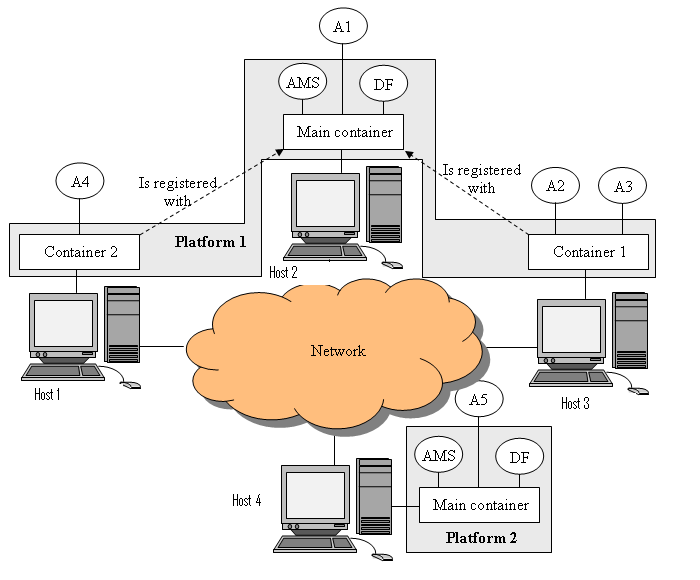
\includegraphics[width=\textwidth]{fig/jadeArchitecture}
	 	\caption{JADE Architechture}
	 	\label{fig:JADEarchitechture}
	 	%Figure found at http://jade.tilab.com/doc/tutorials/JADEAdmin/jadeArchitecture.html
	 	\todo[inline]{Consider remaking this figure so we don't have to cite it}
 \end{figure}

\todo[inline]{Write how we adapted the use of JADE here}


\section{Homomorphic Encryption}
Homomorphic encryption is an encryption scheme which allows computations to be carried out on ciphertext, meaning plaintext that has been encrypted using an algorithm and a public key. The result of the computations is also encrypted, and can be deciphered back to plaintext using a private key. This has long been considered as crypthography's holy grail \cite{Micciancio2011HomoEnc}, as this would allowing operating on encrypted text without knowing the decryption key. For example, given ciphertexts $C_1=Enc(Data1)$ and $C_2=Enc(Data2)$, an additively homomorphic encryption scheme would allow to combine $C_1$ and $C_2$ to obtain $Enc_K(Data1+Data2)$. More concretely this means that if you encrypt your data using such an encryption scheme, you can transfer your data to an untrusted server which can perform some arbitrary computations on that data without being able to decrypt the data itself.

Up until recently, all published homomorphic encryption schemes only supported one basic operation, most commonly addition. These schemes could only be called partially homomorphic, as they did not provide any extensive functionality. The notion of a  fully homomorphic encryption schemes was first proposed by Rivest, Adleman, and Dertouzos in 1978 \cite{rivest1978data}, but it wasn't until 2009 that Craig Gentry published a doctoral thesis where he proved that he had constructed a fully homomorphic scheme\cite{gentry2009FHEpaper}. Gentry's solution was based on "ideal lattices" as well as a method to double-encrypt the data in such a way that the errors could be handled "behind the scenes". By periodically unlocking the inner layer of encryption underneath an outer layer of scrambling, the computer could hide and recover from errors without ever analyzing the secret data. 

\todo{Do we need to talk about a method of HE that doesn't really work for our requirements?}

The downside of Gentry's two-layered approach is that it requires a massive computational effort. Bruce Schneier, a leading American cryptographer, pointed out "Gentry estimates that performing a Google search with encrypted keywords -- a perfectly reasonable simple application of this algorithm -- would increase the amount of computing time by about a trillion. Moore's law calculates that it would be 40 years before that homomorphic search would be as efficient as a search today, and I think he's being optimistic with even this most simple of examples\cite{schneier2009blog}." 


\section{Resource consumption}
\todo{Give analysis of time and space complexities and how much this taxes a device.}


\cleardoublepage
